\documentclass{vgtc}                          % final (conference style)
\usepackage{amsmath}
\usepackage{relsize}
%\documentclass[review]{vgtc}                 % review
%\documentclass[widereview]{vgtc}             % wide-spaced review
%\documentclass[preprint]{vgtc}               % preprint
%\documentclass[electronic]{vgtc}             % electronic version
\newif\ifGPblacktext
\GPblacktexttrue

%% Uncomment one of the lines above depending on where your paper is
%% in the conference process. ``review'' and ``widereview'' are for review
%% submission, ``preprint'' is for pre-publication, and the final version
%% doesn't use a specific qualifier. Further, ``electronic'' includes
%% hyperreferences for more convenient online viewing.

%% Please use one of the ``review'' options in combination with the
%% assigned online id (see below) ONLY if your paper uses a double blind
%% review process. Some conferences, like IEEE Vis and InfoVis, have NOT
%% in the past.

%% Figures should be in CMYK or Grey scale format, otherwise, colour 
%% shifting may occur during the printing process.

%% These three lines bring in essential packages: ``mathptmx'' for Type 1 
%% typefaces, ``graphicx'' for inclusion of EPS figures. and ``times''
%% for proper handling of the times font family.

\usepackage{bm}
\usepackage{mathptmx}
\usepackage{graphicx}
\usepackage{times}


\newcommand*{\SET}[1]  {\ensuremath{\mathcal{#1}}}
\newcommand*{\MAT}[1]  {\ensuremath{\mathbf{#1}}}
\newcommand*{\VEC}[1]  {\ensuremath{\bm{#1}}}
\newcommand*{\CONST}[1]{\ensuremath{\mathit{#1}}}
\newcommand*{\norm}[1]{\mathopen\| #1 \mathclose\|}% use instead of $\|x\|$
\newcommand*{\abs}[1]{\mathopen| #1 \mathclose|}% use instead of $\|x\|$
\newcommand*{\absLR}[1]{\left| #1 \right|}% use instead of $\|x\|$
\newcommand*{\normLR}[1]{\left\| #1 \right\|}% use instead of $\|x\|$

%% We encourage the use of mathptmx for consistent usage of times font
%% throughout the proceedings. However, if you encounter conflicts
%% with other math-related packages, you may want to disable it.

%% If you are submitting a paper to a conference for review with a double
%% blind reviewing process, please replace the value ``0'' below with your
%% OnlineID. Otherwise, you may safely leave it at ``0''.
\onlineid{0}

%% declare the category of your paper, only shown in review mode
\vgtccategory{Research}

%% allow for this line if you want the electronic option to work properly
\vgtcinsertpkg

%% In preprint mode you may define your own headline.
%\preprinttext{To appear in an IEEE VGTC sponsored conference.}

%% Paper title.

\title{SHREC'08 Entry: Shape Based Face Recognition with a Morphable Model}

%% This is how authors are specified in the conference style

%% Author and Affiliation (single author).
%%\author{Roy G. Biv\thanks{e-mail: roy.g.biv@aol.com}}
%%\affiliation{\scriptsize Allied Widgets Research}

%% Author and Affiliation (multiple authors with single affiliations).
%%\author{Roy G. Biv\thanks{e-mail: roy.g.biv@aol.com} %
%%\and Ed Grimley\thanks{e-mail:ed.grimley@aol.com} %
%%\and Martha Stewart\thanks{e-mail:martha.stewart@marthastewart.com}}
%%\affiliation{\scriptsize Martha Stewart Enterprises \\ Microsoft Research}

%% Author and Affiliation (multiple authors with multiple affiliations)
\author{Brian Amberg\thanks{e-mail: \{brian.amberg, reinhard.knothe, thomas.vetter\}@unibas.ch} %
        \and Reinhard Knothe$^*$%
	\and Thomas Vetter$^*$}%

%% Abstract section.
\abstract{
  We present a method for face recognition by fitting a 3D Morphable Model to
  shape data. Fitting is done with a a robust nonrigid ICP algorithm. For
  recognition, it is possible to use either the fitted model parameters, or the
  correspondences induced by the model. We compare different similarity measures,
  and show that a 3D Morphable Model allows very robust retrieval results.
} % end of abstract

%% ACM Computing Classification System (CCS). 
%% See <http://www.acm.org/class/1998/> for details.
%% The ``\CCScat'' command takes four arguments.

\CCScatlist{ 
  \CCScat{I.4.8}{Image Processing and Computer Vision}{Scene Analysis}{Object Recognition, Surface Fitting, Range Data}
  %\CCScat{I.4.7}{Image Processing and Computer Vision}{Feature Measurement}{Size and Shape, Feature representation}
  I.4.7: Feature Measurement---Size and Shape, Feature representation
%  \CCScat{I.4.9}{Image Processing and Computer Vision}{Applications}{}
  I.4.9: Applications
%  \CCScat{I.4.10}{Image Processing and Computer Vision}{Image Representation}{Statistical}
  \CCScat{I.5.1}{Pattern Recognition}{Models}{Statistical}
%  \CCScat{I.5.1}{}{Applications}{Computer Vision}
}

%% Copyright space is enabled by default as required by guidelines.
%% It is disabled by the 'review' option or via the following command:
% \nocopyrightspace

%%%%%%%%%%%%%%%%%%%%%%%%%%%%%%%%%%%%%%%%%%%%%%%%%%%%%%%%%%%%%%%%
%%%%%%%%%%%%%%%%%%%%%% START OF THE PAPER %%%%%%%%%%%%%%%%%%%%%%
%%%%%%%%%%%%%%%%%%%%%%%%%%%%%%%%%%%%%%%%%%%%%%%%%%%%%%%%%%%%%%%%%

\begin{document}

%% The ``\maketitle'' command must be the first command after the
%% ``\begin{document}'' command. It prepares and prints the title block.

%% the only exception to this rule is the \firstsection command
\firstsection{Introduction}

\maketitle

We tackle the task of textureless 3D face recognition. The system is fully
automatic and can handle the typical artifacts of 3D scanners, namely outliers
and missing regions. Face recognition in this setting is a difficult task, and
difficult tasks need strong prior knowledge. To introduce the prior knowledge
we use a 3D Morphable Model (3DMM)~\cite{blanz:model}, which is a generative
statistical model of 3D faces. 3DMM have been applied successfully for face
recognition on different modalities. The most challenging setting is
recognition from single images under varying light and illumination.  This was
adressed by~\cite{blanz03:face_rec,romdhani:recognition}. There a 3DMM with
shape, texture and illumination model was fit to probe and gallery images.  As
the model separates shape and albedo parameters from pose and lighting, it
enables pose and lighting invariant recognition.  In~\cite{amberg07:stereo} a
similar approach was used to fit a pure shape model to stereo images, also
enabling recognition by correlating the shape parameters. We use the same
approach for shape based face recognition. We fit a 3DMM build from 170
subjects with neutral expressions to the \hbox{gavabDB}~\cite{gavabdb} database, and
compare different distance measures which can be derived from the model fit.

An alternative to fitting a generative model is to align the probe to each
example in the database using e.g.\ ICP~\cite{bowyer05:icp_recognition}. But
comparing the probe directly to every gallery image has the disadvantage of
scaling linearly with the number of entries in the gallery, while for a model
based approach only a single fit to the probe is necessary, and the comparision
to the database can then be performed by a distance measure in the lower
dimensional space of registered faces.

Another interesting model-less approach~\cite{bronstein05:face_rec} compares
surface by the distribution of geodesics, which stays constant for nonrigidly
deforming (but not stretching or tearing) objects.  This approach is difficult
to apply in this setting though, as the scanning produces holes, disconnected
regions and strong noise, which can best be handled by a method which uses
specific information about the object class.
			  
\section{Fitting}
\begin{figure}
  \vspace{-0.5em}
  \begin{tabular}{@{ }c@{ }c@{ }c@{ }c@{}}
    \includegraphics[height=0.35\linewidth]{tgt}&
    \includegraphics[height=0.35\linewidth]{src}&
    \includegraphics[height=0.35\linewidth]{step}&
    \includegraphics[height=0.35\linewidth]{extrapolated}\\[-0.8em]
    \smaller a) Target & \smaller b) Fit & \smaller (a) + (b) & \smaller c) Deformed
  \end{tabular}
  \vspace{-1em}
  \caption{The robust fitting gives a good estimate (b) of the true face surface given
  the noisy measurement (a). It fills in holes and removes artifacts using prior
  knowledge from the face model. The fitted shape plus the exact
  correspondences found can be used to extrapolate the image by a robust
  poisson deformation (c).}
  \label{fig:fitting}
\end{figure}
The fitting algorithm used in this paper is a variant of the nonrigid ICP work
in~\cite{amberg07:nicp}. It is a robust iterated fitting algorithm. Like other
ICP methods, it is a local optimization method, which does not guarantee
convergence to the global mimimum, but is dependent on the initialization. It
consists of the following steps
\begin{itemize}
  \item Iterate over a sequence of regularization values $\theta_1>\dots>\theta_N$:
  \begin{itemize}
  \item Repeat until convergence:
    \begin{enumerate}
    \item Find candidate correspondences by searching for the closest compatible
      point for each model vertex.
    \item Weight the correspondences by their distance using a robust estimator.
    \item Fit the 3DMM to these correspondences using a
      regularization strength of $\theta_i$\label{step_fit}.
    \item Continue with the lower $\theta_{i+1}$ if the median change in vertex
      position is smaller than a threshold.
    \end{enumerate}
  \end{itemize}
\end{itemize}
The search for the closest compatible point takes only points into account which
have conforming normals. 
%The search is sped up by organizing the target scan in a space partitioning tree made up of spheres.
%The robust weighting function used in this paper is
%\emph{TODO: Check, what I have really done. I kind of hacked it.}
%\begin{align}
%  w(r) = \left\{\begin{array}{ll} 1+\frac{m_1-r}{m_1}l_0 & \text{if }r<m_1\\\frac{1}{m_2(r-m_1)+1} &\text{otherwise}\end{array}\right.
%\end{align}
%where $m_1$ was set to $3$mm  and $m_2$ to $20$mm. This leads to a robust
%estimation, which discards outliers. 
Note, that it is necessary to balance robustness and regularization, as the
right balance depends on the noise characteristic of the data. Suitable values
were determined manually for a single scan and kept constant for all
experiments.  In step~\ref{step_fit} the 3DMM is fit to 3D-3D point
correspondences.  This is done with a gauss-newton least squares optimization,
using an analytic Jacobian and first-order Hessian.

As the database is pose normalized, we initialize the registration such that
the tip of the nose and pose coincides. This initialization is good enough to
fit the complete database fully automatic. For non pose-normalized databases,
we would either need three landmarks, or -- to keep the algorithm fully
automatic -- repeated random initialization.

\section{Retrieval}
We evaluated four different distance measures, see Figure~\ref{fig:precision} for an overview over their precision recall characteristics.

\subsection{Model Based Measures}
We begin with measures which are acting in the parameter space of the model.
These have the advantage of being extremely cheap to calculate, once the model
has been fit.
\begin{figure}
  \hspace{2.5em}\scalebox{0.68}{% GNUPLOT: LaTeX picture with Postscript
\begingroup
  \fontfamily{phv}%
  \selectfont
  \makeatletter
  \providecommand\color[2][]{%
    \GenericError{(gnuplot) \space\space\space\@spaces}{%
      Package color not loaded in conjunction with
      terminal option `colourtext'%
    }{See the gnuplot documentation for explanation.%
    }{Either use 'blacktext' in gnuplot or load the package
      color.sty in LaTeX.}%
    \renewcommand\color[2][]{}%
  }%
  \providecommand\includegraphics[2][]{%
    \GenericError{(gnuplot) \space\space\space\@spaces}{%
      Package graphicx or graphics not loaded%
    }{See the gnuplot documentation for explanation.%
    }{The gnuplot epslatex terminal needs graphicx.sty or graphics.sty.}%
    \renewcommand\includegraphics[2][]{}%
  }%
  \providecommand\rotatebox[2]{#2}%
  \@ifundefined{ifGPcolor}{%
    \newif\ifGPcolor
    \GPcolortrue
  }{}%
  \@ifundefined{ifGPblacktext}{%
    \newif\ifGPblacktext
    \GPblacktextfalse
  }{}%
  % define a \g@addto@macro without @ in the name:
  \let\gplgaddtomacro\g@addto@macro
  % define empty templates for all commands taking text:
  \gdef\gplbacktext{}%
  \gdef\gplfronttext{}%
  \makeatother
  \ifGPblacktext
    % no textcolor at all
    \def\colorrgb#1{}%
    \def\colorgray#1{}%
  \else
    % gray or color?
    \ifGPcolor
      \def\colorrgb#1{\color[rgb]{#1}}%
      \def\colorgray#1{\color[gray]{#1}}%
      \expandafter\def\csname LTw\endcsname{\color{white}}%
      \expandafter\def\csname LTb\endcsname{\color{black}}%
      \expandafter\def\csname LTa\endcsname{\color{black}}%
      \expandafter\def\csname LT0\endcsname{\color[rgb]{1,0,0}}%
      \expandafter\def\csname LT1\endcsname{\color[rgb]{0,1,0}}%
      \expandafter\def\csname LT2\endcsname{\color[rgb]{0,0,1}}%
      \expandafter\def\csname LT3\endcsname{\color[rgb]{1,0,1}}%
      \expandafter\def\csname LT4\endcsname{\color[rgb]{0,1,1}}%
      \expandafter\def\csname LT5\endcsname{\color[rgb]{1,1,0}}%
      \expandafter\def\csname LT6\endcsname{\color[rgb]{0,0,0}}%
      \expandafter\def\csname LT7\endcsname{\color[rgb]{1,0.3,0}}%
      \expandafter\def\csname LT8\endcsname{\color[rgb]{0.5,0.5,0.5}}%
    \else
      % gray
      \def\colorrgb#1{\color{black}}%
      \def\colorgray#1{\color[gray]{#1}}%
      \expandafter\def\csname LTw\endcsname{\color{white}}%
      \expandafter\def\csname LTb\endcsname{\color{black}}%
      \expandafter\def\csname LTa\endcsname{\color{black}}%
      \expandafter\def\csname LT0\endcsname{\color{black}}%
      \expandafter\def\csname LT1\endcsname{\color{black}}%
      \expandafter\def\csname LT2\endcsname{\color{black}}%
      \expandafter\def\csname LT3\endcsname{\color{black}}%
      \expandafter\def\csname LT4\endcsname{\color{black}}%
      \expandafter\def\csname LT5\endcsname{\color{black}}%
      \expandafter\def\csname LT6\endcsname{\color{black}}%
      \expandafter\def\csname LT7\endcsname{\color{black}}%
      \expandafter\def\csname LT8\endcsname{\color{black}}%
    \fi
  \fi
  \setlength{\unitlength}{0.0500bp}%
  \begin{picture}(6242.40,2016.00)%
    \gplgaddtomacro\gplbacktext{%
      \csname LTb\endcsname%
      \put(129,216){\makebox(0,0)[r]{\strut{} 0}}%
      \csname LTb\endcsname%
      \put(129,540){\makebox(0,0)[r]{\strut{} 0.2}}%
      \csname LTb\endcsname%
      \put(129,864){\makebox(0,0)[r]{\strut{} 0.4}}%
      \csname LTb\endcsname%
      \put(129,1188){\makebox(0,0)[r]{\strut{} 0.6}}%
      \csname LTb\endcsname%
      \put(129,1512){\makebox(0,0)[r]{\strut{} 0.8}}%
      \csname LTb\endcsname%
      \put(129,1836){\makebox(0,0)[r]{\strut{} 1}}%
      \csname LTb\endcsname%
      \put(237,36){\makebox(0,0){\strut{} 0}}%
      \csname LTb\endcsname%
      \put(1416,36){\makebox(0,0){\strut{} 0.2}}%
      \csname LTb\endcsname%
      \put(2596,36){\makebox(0,0){\strut{} 0.4}}%
      \csname LTb\endcsname%
      \put(3775,36){\makebox(0,0){\strut{} 0.6}}%
      \csname LTb\endcsname%
      \put(4955,36){\makebox(0,0){\strut{} 0.8}}%
      \csname LTb\endcsname%
      \put(6134,36){\makebox(0,0){\strut{} 1}}%
      \put(-450,1026){\rotatebox{90}{\makebox(0,0){\strut{}Precision}}}%
      \put(3185,-100){\makebox(0,0){\strut{}Recall}}%
      \put(3185,1746){\makebox(0,0){\strut{}}}%
    }%
    \gplgaddtomacro\gplfronttext{%
      \csname LTb\endcsname%
      \put(2505,909){\makebox(0,0)[r]{\strut{}Mahalanobis Distance}}%
      \csname LTb\endcsname%
      \put(2505,729){\makebox(0,0)[r]{\strut{}Mahalanobis Angle}}%
      \csname LTb\endcsname%
      \put(2505,549){\makebox(0,0)[r]{\strut{}Vertex Distance}}%
      \csname LTb\endcsname%
      \put(2505,369){\makebox(0,0)[r]{\strut{}Geodesic}}%
    }%
    \gplbacktext
    \put(0,0){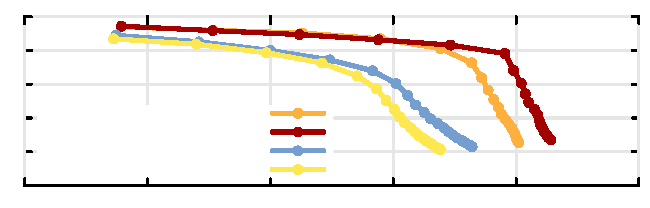
\includegraphics{precision_recall}}%
    \gplfronttext
  \end{picture}%
\endgroup
}
  \vspace{-0.7em}
  \caption{Measures in Mahalanobis Space outperform vertex based measures.}
  \label{fig:precision}
\end{figure}
\begin{figure}
  \vspace{-1.0em}
  \hspace{2.5em}\scalebox{0.68}{% GNUPLOT: LaTeX picture with Postscript
\begingroup
  \fontfamily{phv}%
  \selectfont
  \makeatletter
  \providecommand\color[2][]{%
    \GenericError{(gnuplot) \space\space\space\@spaces}{%
      Package color not loaded in conjunction with
      terminal option `colourtext'%
    }{See the gnuplot documentation for explanation.%
    }{Either use 'blacktext' in gnuplot or load the package
      color.sty in LaTeX.}%
    \renewcommand\color[2][]{}%
  }%
  \providecommand\includegraphics[2][]{%
    \GenericError{(gnuplot) \space\space\space\@spaces}{%
      Package graphicx or graphics not loaded%
    }{See the gnuplot documentation for explanation.%
    }{The gnuplot epslatex terminal needs graphicx.sty or graphics.sty.}%
    \renewcommand\includegraphics[2][]{}%
  }%
  \providecommand\rotatebox[2]{#2}%
  \@ifundefined{ifGPcolor}{%
    \newif\ifGPcolor
    \GPcolortrue
  }{}%
  \@ifundefined{ifGPblacktext}{%
    \newif\ifGPblacktext
    \GPblacktextfalse
  }{}%
  % define a \g@addto@macro without @ in the name:
  \let\gplgaddtomacro\g@addto@macro
  % define empty templates for all commands taking text:
  \gdef\gplbacktext{}%
  \gdef\gplfronttext{}%
  \makeatother
  \ifGPblacktext
    % no textcolor at all
    \def\colorrgb#1{}%
    \def\colorgray#1{}%
  \else
    % gray or color?
    \ifGPcolor
      \def\colorrgb#1{\color[rgb]{#1}}%
      \def\colorgray#1{\color[gray]{#1}}%
      \expandafter\def\csname LTw\endcsname{\color{white}}%
      \expandafter\def\csname LTb\endcsname{\color{black}}%
      \expandafter\def\csname LTa\endcsname{\color{black}}%
      \expandafter\def\csname LT0\endcsname{\color[rgb]{1,0,0}}%
      \expandafter\def\csname LT1\endcsname{\color[rgb]{0,1,0}}%
      \expandafter\def\csname LT2\endcsname{\color[rgb]{0,0,1}}%
      \expandafter\def\csname LT3\endcsname{\color[rgb]{1,0,1}}%
      \expandafter\def\csname LT4\endcsname{\color[rgb]{0,1,1}}%
      \expandafter\def\csname LT5\endcsname{\color[rgb]{1,1,0}}%
      \expandafter\def\csname LT6\endcsname{\color[rgb]{0,0,0}}%
      \expandafter\def\csname LT7\endcsname{\color[rgb]{1,0.3,0}}%
      \expandafter\def\csname LT8\endcsname{\color[rgb]{0.5,0.5,0.5}}%
    \else
      % gray
      \def\colorrgb#1{\color{black}}%
      \def\colorgray#1{\color[gray]{#1}}%
      \expandafter\def\csname LTw\endcsname{\color{white}}%
      \expandafter\def\csname LTb\endcsname{\color{black}}%
      \expandafter\def\csname LTa\endcsname{\color{black}}%
      \expandafter\def\csname LT0\endcsname{\color{black}}%
      \expandafter\def\csname LT1\endcsname{\color{black}}%
      \expandafter\def\csname LT2\endcsname{\color{black}}%
      \expandafter\def\csname LT3\endcsname{\color{black}}%
      \expandafter\def\csname LT4\endcsname{\color{black}}%
      \expandafter\def\csname LT5\endcsname{\color{black}}%
      \expandafter\def\csname LT6\endcsname{\color{black}}%
      \expandafter\def\csname LT7\endcsname{\color{black}}%
      \expandafter\def\csname LT8\endcsname{\color{black}}%
    \fi
  \fi
  \setlength{\unitlength}{0.0500bp}%
  \begin{picture}(6242.40,1512.00)%
    \gplgaddtomacro\gplbacktext{%
      \csname LTb\endcsname%
      \put(129,72){\makebox(0,0)[r]{\strut{} 0}}%
      \csname LTb\endcsname%
      \put(129,282){\makebox(0,0)[r]{\strut{} 0.05}}%
      \csname LTb\endcsname%
      \put(129,492){\makebox(0,0)[r]{\strut{} 0.1}}%
      \csname LTb\endcsname%
      \put(129,702){\makebox(0,0)[r]{\strut{} 0.15}}%
      \csname LTb\endcsname%
      \put(129,912){\makebox(0,0)[r]{\strut{} 0.2}}%
      \csname LTb\endcsname%
      \put(129,1122){\makebox(0,0)[r]{\strut{} 0.25}}%
      \csname LTb\endcsname%
      \put(129,1332){\makebox(0,0)[r]{\strut{} 0.3}}%
      \csname LTb\endcsname%
      \put(237,-108){\makebox(0,0){\strut{} 0.2}}%
      \csname LTb\endcsname%
      \put(1220,-108){\makebox(0,0){\strut{} 0.4}}%
      \csname LTb\endcsname%
      \put(2203,-108){\makebox(0,0){\strut{} 0.6}}%
      \csname LTb\endcsname%
      \put(3185,-108){\makebox(0,0){\strut{} 0.8}}%
      \csname LTb\endcsname%
      \put(4168,-108){\makebox(0,0){\strut{} 1}}%
      \csname LTb\endcsname%
      \put(5151,-108){\makebox(0,0){\strut{} 1.2}}%
      \csname LTb\endcsname%
      \put(6134,-108){\makebox(0,0){\strut{} 1.4}}%
      \put(-450,702){\rotatebox{90}{\makebox(0,0){\strut{}Frequency}}}%
      \put(3185,-280){\makebox(0,0){\strut{}Distance}}%
      \put(3185,1242){\makebox(0,0){\strut{}}}%
    }%
    \gplgaddtomacro\gplfronttext{%
      \csname LTb\endcsname%
      \put(1209,1179){\makebox(0,0)[r]{\strut{}Match}}%
      \csname LTb\endcsname%
      \put(1209,999){\makebox(0,0)[r]{\strut{}Impostor}}%
    }%
    \gplbacktext
    \put(0,0){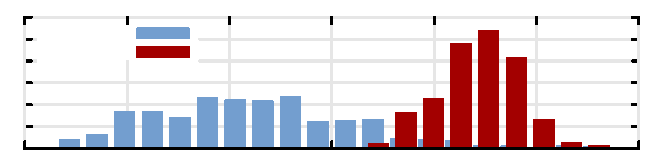
\includegraphics{impostor}}%
    \gplfronttext
  \end{picture}%
\endgroup
}
  \vspace{0.1em}
  \caption{Impostor detection is reliable, as the minimum distance to a match is smaller than the minimum distance to a nonmatch.}
  \label{fig:impostor}
\end{figure}

\subsubsection{Mahalanobis distance of shape coefficients}
%\paragraph{Mahalanobis distance of shape coefficients}
The first method calculates the distance between two vectors of shape
coefficients $\VEC \alpha_1$ and $\VEC\alpha_2$ expressed in Mahalanobis space
as
\begin{align}
  s_1(\VEC\alpha_1, \VEC\alpha_2) &= \norm{\VEC\alpha_1 - \VEC\alpha_2}\qquad.
\end{align}

\subsubsection{Angular distance of shape coefficients}
In face space, caricatures lie along the rays from the origin.
Mapping all caricatured versions of a face onto a canonical face gives a method
which has proven to have very high recognition rates~\cite{blanz03:face_rec}.
To do this we use the angle between the shape coefficients in Mahalanobis space
as the distance measure:
\begin{align}
  s_2(\VEC\alpha_1, \VEC\alpha_2) &= \arccos\left(\frac{\VEC\alpha_1^T\VEC\alpha_2}{\norm{\VEC\alpha_1}\norm{\VEC\alpha_2}}\right)\qquad.
\end{align}
For the angular measure shown in Figure~\ref{fig:impostor} the distribution of
distances towards the first match and the first nonmatch in the database. This
shows, that by choosing a suitable threshold it is possible to perform face
recognition with impostors, where we decide if the identity is in the database
or not.

These two measures give similar results, but the caricature invariance of the
angular distance improves recall a bit. This tells us, that in face space, the
direction alone codes the identity.

\subsection{Shape Based Measures}
The second type of measures acts in vertex space. If we want to compare
two model instances, it does not make much sense to measure in vertex space
instead of parameter space, as there is a one to one mapping between the spaces
and the parameter space is of much lower dimensionality. But in our case we do
have additional information which can not be expressed by the model.
After fitting, some residual will remain, which is caused by three reasons. 1)
The individuals used to train the model were not from the gallery, and we can
not span the complete face space with 170 training examples.  2) The probe
images have expressions, while the database was build using neutral expressions.
3) The aquisition process introduces noise. Therefore, we add more
flexibility to the model by allowing smooth nonrigid deformations of the final
fit to minimize the remaining residual. This is achieved by robustly fitting a
poisson deformation with soft boundary and zero right hand side, where the
boundary is given by the correspondences found by the fitting algorithm, and
the deformed shape is the fitted head.  Results can be seen in
Figure~\ref{fig:fitting}.  With these correspondence established we can use
different distance measures.

\subsubsection{Distance}
Denote the $N$ vertices of the registered scan $i$ as $\VEC v^i_1,\dots,\VEC
v^i_N$.  We use the distance after removing the rigid transformation, measuring
only in a mask defined on the model, which includes the parts which are visible
in most of the scans. We compute
\begin{align}
  s_3(\MAT v^1, \MAT v^2)  &= \min_{\MAT R,\VEC t} \sum_i \norm{\MAT R\VEC v^1_i + \VEC t - \VEC v^2_i}\qquad.
\end{align}
where $\MAT R,\VEC t$ describe a similarity transform.
%
While this measure is straight forward, the recognition results are
unsatisfying. The scaling of face space which is learned from the example faces
results in an improved clustering of scans, which enables better classification
than comparisions in the original vertex space.

\subsubsection{Geodesics}
Inspired by~\cite{bronstein05:face_rec} we tried a geodesic based measure,
which should be invariant against expression changes. We classify by comparing
the distances of a selected set of vertices, which were assumed not to change
under expressions.  Denote the selected vertex pairs by $\SET P$. Note that
this is different from~\cite{bronstein05:face_rec}, as we have already brought
the meshes into correspondence during fitting. The measure is then
\begin{align}
  s_4(\MAT v^1, \MAT v^2) &= \sum_{(i,j)\in \SET P} \absLR{ \norm{v^1_i - v^1_j} - \norm{v^2_i - v^2_j}}
\end{align}
Experiments with different sets of distances showed that the best
classification results were achieved by selecting all neighboring edges of the
model in the face area. Still, exactly because this method introduces some
invariance, it also reduces the precision in the retrieval experiments. Also,
it does not incorporate the knowledge about face space, which was exploited in
the first two methods.

\section{Conclusion}
We have shown that 3D Morphable Models provide a valuable tool for face
recognition with 98.8\% recognition rate on this database. The strong prior
knowledge allows robust handling of noisy data. Four distance measures
were compared, and it turns out that the angular distance in Mahalanobis space
is the most accurate classifier. It was noticably better than measuring
the difference between the registered scans. This is because the face space
learned from our training examples is constructed such that the identities are
better separated than in vertex space.

In the future we wish to make the system expression invariant, by using a
model which separates expression and identity. As we do establish
correspondence between the model and the scans, it is trivial to add image
based classification for datasets where a calibrated photo is available, by
comparing the rectified textures.

%% if specified like this the section will be ommitted in review mode
\acknowledgements{The authors wish to thank P.\ Paysan for the data
acquisition. This work was supported in part by a grant from Microsoft
Research and the Swiss National Science Foundation (200021-103814 and NCCR COME project 5005-66380).}

\bibliographystyle{abbrv}
%%use following if all content of bibtex file should be shown
%\nocite{*}
\bibliography{shrec_08}
\end{document}
